\section{Iterative Problems}
\subsection{Brute-Force}

Brute force problems are best described as problems where the intended (or at least, a valid) solution involves trying every possibility. These are usually marked by very small problem bounds, because of how computationally complex this process can be.

What exactly brute-force looks like depends on the problem itself. In some cases, it's "try all pairs" which is $O(n^2)$. It can be "try all triplets" at $O(n^3)$. Sometimes it's all combinations, in $O(2^n)$. In some cases, it's try all permutations which is $O(n!)$.

There is a reason we distinguish brute-force \textit{problems} from brute-force \textit{solutions}. For most problems, it's possible to find a brute-force solution that is guaranteed to give you the right answer. Usually it's pretty easy to come up with a technically valid brute-force solution, in fact. Most problems can't be solved with this approach because it tends to be extremely slow. A brute-force problem is a problem where the brute-force solution is valid and can work.

\subsection{Simulation}

Simulation problems are problems where the problem description describes some step-by-step algorithm (and the algorithm may be a single step repeated some number of times), and the intended solution is to simply perform that algorithm.

Generally, the difficulty from simulation problems comes from how difficult their implementation is, not from figuring out the solution. They tend to be relatively straightforward to understand a solution for (the problem statement tells you the solution, in a sense) but can be difficult to convert into code. Sometimes, the implementation details matter and while you're still just implementing what the problem statement tells you to do, you have to consider what data structures you're using in order to pass the time constraints on the problem.

We'll look at a simulation problem that involves a mathematical concept "Happy Numbers". Despite looking math-related, a simulation approach is the recommended solution.

\hrulefill

\problem{Very Happy}
{If you take a positive integer and sum the square of all its digits, you end up with an interesting transformation. For example, applying this to $123$ gives us $1^2 + 2^2 + 3^2 = 14$.

We can repeat this process multiple times, such as taking $14$ and getting $1^2 + 4^2 = 17$, $17$ becoming $1^2 + 7^2 = 50$, $50$ becoming $25$, $25$ becoming $29$, becoming $85$, then $89$, then $145$, then $42$, $20$, then $4$. This will continue to loop forever, since it turns out that $4$ enters a cycle $4,16,37,58,89,145,42,20,4$.

Not all numbers will enter into a long cycle when you do this -- some numbers will turn into $1$ when you repeat this process enough times (and applying this process on $1$ gives us $1^2 = 1$). These are called happy numbers.

The task here is to determine whether a number is happy or not. And if it is happy, figure out how many iterations it takes to do so.}
{Input consists of an integer $1 \le t \le 10^5$. Then follows $t$ integers $1 \le n \le 10^9$.}
{For every integer $n$, output either the number of iterations it takes to become $1$, or "impossible" if it never does.}
{1 second}
{1024 mb}
{\IOsample{problems/very_happy/1}}

\hrulefill

\subsection{Two-Pointers}

Two-pointers problems, generally speaking, are problems that can be solved by keeping track of two locations on a sorted array. One pointer starts at the start of the array (the smallest element) and the other starts at the end of the array (the largest element). You are asked to find a pair of elements for which a certain property holds.

A classic example is "given a sorted array of integers, determine whether a pair of elements sums up to 100".

It is simple to solve this problem using a brute-force approach in $O(n^2)$:

\inputcpp{code/iterative/find-sum-brute-force.cpp}

It can be improved further by using binary search instead our nested for loop, which turns it $O(n log n)$ instead:

\inputcpp{code/iterative/find-sum-binary-search.cpp}

But with a two-pointers approach we can perform this in $O(n)$:

\inputcpp{code/iterative/find-sum-two-pointers.cpp}

To explain how this works internally, let's consider an array $1,2,7,49,50,51,95,100,110$. We start with considering the first and last elements, and then we will repeatedly perform this:
\begin{enumerate}
\item $1 + 110 = 111$, which is greater than $100$ so we decrease right
\item $1 + 100 = 101$, which is greater than $100$ so we decrease right
\item $1 + 95 = 96$, which is less than $100$ so we increase left
\item $2 + 95 = 97$, which is less than $100$ so we increase left
\item $7 + 95 = 102$, which is greater than $100$ so we decrease right
\item $7 + 51 = 58$, which is less than $100$ so we increase left
\item $49 + 51 = 100$, which is our target value, so we return true
\end{enumerate}

It's useful to compare with an array that doesn't have a correct answer, like $1,5,97,100$:
\begin{enumerate}
\item $1 + 100 = 101$, which is greater than $100$ so we decrease right
\item $1 + 97 = 98$, which is less than $100$ so we increase left
\item $5 + 97 = 102$, which is greater than $100$ so we decrease right
\item both pointers are at the second element, so we return false
\end{enumerate}

There's two things to note about this approach: it relies on the array being sorted (if it isn't sorted, you must sort it first), and that you at every step of the way, you either:
\begin{itemize}
\item found a valid pair
\item know that your left pointer is too small (because your sum is too low, and changing the right pointer will only decrease it further)
\item know that your right pointer is too high (because your sum is too high, and changing your left pointer will only increase it further)
\end{itemize}

\subsection{Sliding Window}

In a sliding window problem, we have a list of elements, and we want to find a range of a certain length with some property.

Consider a problem like "given an array of integers, determine whether a subarray of length $k$ sums to 100". This isn't too hard to think of conceptually, and we can solve it with a straightforward brute-force approach -- sum all elements from $[0,k)$ and see if they equal 100, then sum from $[1,k+1)$ and see if they equal 100, and so on.

You'll notice that we redo a lot of work with that brute-force approach. Both $[0,k)$ and $[1,k+1)$ involve the sum $[1,k)$, so we can reduce the amount of operations we need to do if we can stop re-adding elements together unnecessarily.

With a sliding window, we can move from $[0,k)$ to $[1,k+1)$ by subtracting $arr[0]$ and adding $arr[k]$, so that we now have our next range in two operations instead of $k$ operations.

\subsubsection{Resizing Window}

You can combine concepts with two-pointers and sliding windows together, where you keep left and right pointers like with two-pointers, but instead of considering pairs we consider ranges like with sliding windows.

A classical example for this is "given an array of non-negative integers, determine whether any subarray sums to 100". We approach this by starting with a range that's only the first element, and then if it's too small we add the element to the right of our window, and if it's too large we subtract the element at the left.

For example, let's look at the array $20,30,5,5,50,30,5,5,80,20$. If we want to find a subarray that sums to 100, we can look:

{\centering 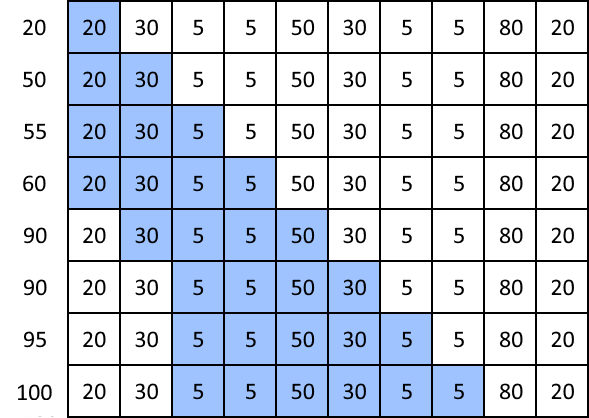
\includegraphics[width=\textwidth]{images/iterative/resizing-window}}

Where the cells shaded blue are the current subarray we're considering, and the number to the left represents the current sum of the entire range. We find our final answer to be the subarray $5,5,50,30,5,5$.

Note that in this example problem we're just looking for whether or not there is a subarray that sums to 100. If we want to find all subarrays that sum to 100, or the smallest such subarray (in our above example, the last two elements $80,20$ sum to 100 in a mich smaller subarray), or some other criteria, we can still use the resizing window approach but will have to prevent it from finishing as soon as we find a valid range.

There are various ways to implement this. Here's an example implementation that used a for-loop for the left pointer, and a nested while-loop for the right pointer.

\inputcpp{code/iterative/subarray-sum-resizing-window.cpp}

Something a keen eye might've noticed is that our example problem was "non-negative integers". This was carefully chosen, because this approach doesn't work when we include the possibility of negative numbers. Specifically, the sliding window technique relies on increasing the window size to always either increase our sum or keep it the same, and likewise that decreasing the window size will always decrease our sum or keep it the same. This assumption doesn't hold with negatives numbers.

To demonstrate the problem with negative numbers, let's look at the counter-example $50, -1, 50, 50, -99$. It should be obvious that there is a subarray that sums to 100, specially the $50,50$ in the middle. If we attempt to find this via a resizing window, we will instead get:
\begin{enumerate}
\item our range is $50$ with sum $50$, which is less than 100 so we increase our window size
\item our range is $50,-1$ with sum $49$, which is less than 100 so we increase our window size
\item our range is $50,-1,50$ with sum $99$, which is less than 100 so we increase our window size
\item our range is $50,-1,50,50$ with sum $149$, which is greater than 100 so we decrease our window size
\item our range is $-1,50,50$ with sum $99$, which is less than 100 so we increase our window size
\item our range is $-1,50,50,-99$ with sum $0$, which is less than 100 so we increase our window size, except that we have traversed the entire array and have no more elements to consider
\end{enumerate}

\subsection{Constructive}

Sometimes you will find problems along the lines of "here is a list of restrictions, construct an array that meets those restrictions" or "create the optimum answer under a list of restrictions". Usually, they also have some variant on "if there are multiple solutions, print any of them."

Generally, constructive problems require creative thinking to figure out a valid pattern that will satisfy the requirements. Usually, the implementation of a valid program itself is not very complicated, and it's being able to determine a valid pattern that is the challenging and interesting part of the problem.

Constructive problems are not necessarily iterative, but it's reasonable to introduce constructive problems here because many of them are.

We'll look at an example of a constructive problem:

\hrulefill

\problem{Big Difference}
{"Big Difference!" Ivan said to his teacher, pointing at a list of numbers the teacher wrote on the board.

"That's right Ivan, there is a big difference here", the teacher said pointing to how the difference between every two elements in the list is fairly large. "In fact, I had carefully ensured that the difference between all elements was as large as possible, so that no elements next to each other was small." Specifically, the teacher made a list where the smallest (absolute) difference between every adjacent element was as large as possible.

Ivan wanted to figure out how to do this, but was not very fast at it. He couldn't figure out a way to solve it other than trying every different arrangement of the list, which was far too slow when he had a large list to deal with.}
{Input consists of a single integer $n$ where $1 \le n \le 10^8$.}
{Output an list of numbers of size $n$ with values $[1,2,3,...,n]$ where the smallest absolute difference between adjacent elements is maximized. More formally, create a permutation of an array $a$ with values $[1,n]$ with the maximum value of $min(|a_1-a_2|, |a_2-a_3|, ... |a_{n-1}-a_{n}|)$. If there are multiple answers, print any.}
{1 second}
{1024 mb}
{\IOsample{problems/big_difference/1}
\IOsample{problems/big_difference/2}}

\hrulefill

There's a few things about this problem that stands out. The restriction is fairly basic -- we just have to make sure the minimum difference between adjacent elements is as large as possible. Our output is just a list of numbers between $1$ and $n$ that's ordered in a way that meets this restriction.

There can be multiple variants on this problem. It could also provide an input $k$ and ask that no two adjacent elements have an absolute difference less than $k$. It could ask for the lexicographically smallest answer if there are multiple (if $2 1 3$ and $3 1 2$ as both valid answers, the lexicographically smallest answer would be $2 1 3$ since $2$ is less than $3$).

It's worth mentioning that it's rare for the sample inputs/outputs to actually describe each possible different valid answer for a given input. It's also unlikely that the test cases will show particularly large test cases. The reason for both of these is that a valid pattern may become obvious with this information. The sample cases are usually carefully chosen so that it's clear what the IO expects and can clarify what the problem expects, but doesn't give you any strong leads into what a solution might look like.
